\documentclass[dvipdfmx, fleqn]{jsarticle}
\input{/Users/User/Documents/University/report_template/preamble/preamble}
\title{
    パターン認識 最終レポート \\
    FaceNet: A Unified Embedding for Face Recognition and Clustering
    }
\author{37-196360 \quad 森田涼介}
\bibliographystyle{junsrt}
\begin{document}
\maketitle

\section{論文の概要}

FaceNet\cite{schroff2015facenet}についての概要を記す。


\subsection{サマリー}

\begin{itemize}
    \item Bibliography
    \begin{itemize}
        \item Paper: \href{https://ieeexplore.ieee.org/document/7298682}{FaceNet: A unified embedding for face recognition and clustering}
        \item Date: 2015-06-12
        \item Authors: Florian Schroff, Dmitry Kalenichenko, James Philbin
        \item Published in: 2015 IEEE Conference on Computer Vision and Pattern Recognition (CVPR)
    \end{itemize}
    \item Keywords
    \begin{itemize}
        \item face verification
        \item face recognition
        \item face clustering
        \item deep convolutional network
        \item triplet loss
    \end{itemize}
    \item Model
    \begin{itemize}
        \item Name: FaceNet
        \item Input: Face Image (e.g. \num{224 x 224 x 3})
        \item Output: Embedding (128-D)
        \item Network: CNN (e.g. Inception)
        \item Loss: Triplet Loss
    \end{itemize}
    \item Dataset
    \begin{itemize}
        \item Labelled Faces in the Wild (LWF)
        \item YouTube Faces
    \end{itemize}
    \item Points of view
    \begin{itemize}
        \item DCNNで顔画像を128次元のembeddingsに変換
        \item embedding間のEuclid距離が,顔の類似度に対応
        \begin{itemize}
            \item 距離が近いほど似ている
            \item 顔認証,顔認識,顔画像のクラスタリングにそのまま使える
        \end{itemize}
        \item Triplet Lossを用い,同一人物の顔画像のembeddingsは近く,異なる人のembeddingsは遠くなるように訓練
        \item Tripletの作り方を工夫し,lossの収束に効くような組み合わせを選ぶ
        \item 2画像が同一人物かどうかの二値分類の正解率は,LWFが99.63{\%},YouTube Facesが95.12{\%}でSOTAを達成
    \end{itemize}
\end{itemize}


\subsection{理論}

画像\(x\)のembeddingを\(f(x)\ (\in \mathbb{R}^{d})\)と表す。
\(f\)は\(x\)を\(d\)次元のEuclid空間に写像する。
また,embeddingを\(d\)次元の超球上に制限する(\(||f(x)||_2 = 1\))。
ある人の顔画像\(x_i^\mathrm{a}\ (\text{anchor})\)と
その人の他の画像\(x_i^\mathrm{p}\ (\text{positive})\)との距離が,
他の人の画像\(x_i^\mathrm{n}\ (\text{negative})\)との距離より小さくなるように学習したい。
式で表すと,
\begin{align}
    & ||f(x_i^\mathrm{a}) - f(x_i^\mathrm{p})||_2^2 + \alpha < ||f(x_i^\mathrm{a}) - f(x_i^\mathrm{n})||_2^2
    \label{eq:wanted} \\
    & \forall \qty(f(x_i^\mathrm{a}),\ f(x_i^\mathrm{p}),\ f(x_i^\mathrm{n})) \in \mathscr{T}
    \label{eq:triplets}
\end{align}
ここで,\(\alpha\)はマージンで,
\(\mathscr{T}\)は訓練データにおけるtripletの組み合わせである(\(||\mathscr{T}|| = N\))。
損失関数は,
\begin{equation}
    \mathscr{L} = \sum_{i}^{N} \qty[||f(x_i^\mathrm{a}) - f(x_i^\mathrm{p})||_2^2 - ||f(x_i^\mathrm{a}) - f(x_i^\mathrm{n})||_2^2 + \alpha]_{+}
    \label{eq:loss}
\end{equation}
となる。

Tripletの選択について議論する。
考えうる全てのtripletの組み合わせを生成しても,
式(\ref{eq:wanted})が満たされているような組み合わせは学習に貢献しないため,
ただ学習時間を増加させるだけになってしまう。
そこで,式(\ref{eq:wanted})を満たさないようなtrpiletを選択することを考える。
つまり,あるanchor画像\(x_i^\mathrm{a}\)に対して,
次のような\(x_i^\mathrm{p},\ x_i^\mathrm{n}\)を選ぶ。
\begin{align*}
    & x_i^\mathrm{p} = \arg\max_{x_i^\mathrm{p}} ||f(x_i^\mathrm{a}) - f(x_i^\mathrm{p})||_2^2 \\
    & x_i^\mathrm{n} = \arg\min_{x_i^\mathrm{n}} ||f(x_i^\mathrm{a}) - f(x_i^\mathrm{n})||_2^2
\end{align*}
しかし,\(\arg\max,\ \arg\min\)を全訓練データに対して計算するのは,
計算時間やデータの質(ラベルの誤りや画像の質)を考えれば妥当ではない。
そこで,ミニバッチの中で\(\arg\max,\ \arg\min\)を考える。
このとき,ミニバッチの中には,1人につき2枚以上の画像が必要である。
ただし,anchor-positiveに関しては,\(\arg\max\)でなく全組み合わせを考えてもよい。
また,\(\arg\min\)となるような\(x_i^\mathrm{n}\)を選ぶと学習初期に悪い局所最適解,
特に\(f(x) = 0\)に収束してしまうことがある。
そのため,
\begin{equation}
    ||f(x_i^\mathrm{a}) - f(x_i^\mathrm{p})||_2^2 < ||f(x_i^\mathrm{a}) - f(x_i^\mathrm{n})||_2^2
\end{equation}
を満たすような\(x_i^\mathrm{n}\)を選ぶとよい。


\begin{figure}[H]
    \centering
    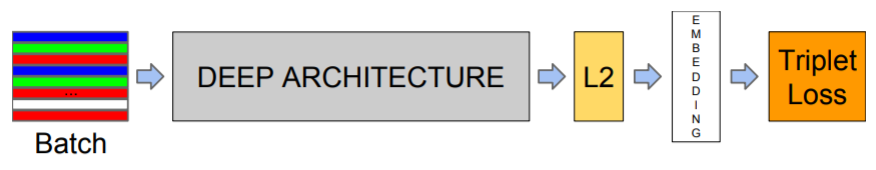
\includegraphics[clip, width=15cm]{./figures/model_structure}
    \caption{モデルの構造}
    \label{fig:model_structure}
\end{figure}


\begin{figure}[H]
    \centering
    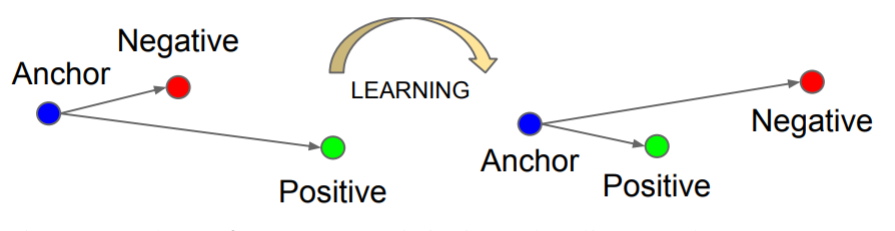
\includegraphics[clip, width=15cm]{./figures/triplet_loss}
    \caption{Triplet Loss}
    \label{fig:triplet_loss}
\end{figure}



\section{扱う問題と評価指標}

顔認識・顔認証・顔画像のクラスタリングといった問題を扱う。
顔認識・顔認証は,セキュリティや犯罪捜査など様々な場面で重要となる技術である。
本論文では,顔画像をembeddingに変換し,
それらの距離を測ることでこれらの問題を解決している。
すなわち,embedding同士が近ければ似ており,
遠ければ似ていないというようにして解いている。
学習にはTripet Lossを用いていて,
同一人物の顔画像のembeddingを近く,
異なる人物の顔画像のembeddingを遠くするように最適化する。

評価方法について考える。
\(x_i\)と\(x_j\)の間の距離を\(D(x_i,\ x_j)\),
同一人物かどうかの閾値を\(d\)とし,
同一人物の画像のペアを\(\mathscr{P}_\mathrm{same}\),
異なる人物の画像のペアを\(\mathscr{P}_\mathrm{diff}\)とする。
同一人物のペアのうち,正しく同一人物であると判定された,
true acceptsのペアの集合を次のように表す。
\begin{equation}
    \mathrm{TA}(d) = \qty{(i,\ j) \in \mathscr{P}_\mathrm{same},\ D(x_i,\ x_j) \le d}
\end{equation}
また,異なる人物のペアのうち同一人物であると判定された,
false acceptsのペアの集合を次のように表す。
\begin{equation}
    \mathrm{FA}(d) = \qty{(i,\ j) \in \mathscr{P}_\mathrm{diff},\ D(x_i,\ x_j) \le d}
\end{equation}
これらを用いて,次の2つの評価指標を導入する。
\begin{equation}
    \mathrm{VAL}(d) = \frac{|\mathrm{TA}(d)|}{|\mathscr{P}_\mathrm{same}|}
    , \qquad
    \mathrm{FAR}(d) = \frac{|\mathrm{FA}(d)|}{|\mathscr{P}_\mathrm{diff}|}
\end{equation}
\(\mathrm{VAL}(d)\)が高く,\(\mathrm{FAR}(d)\)が低いほど性能が良い。



\section{論文の選定理由}

画像のembeddingを得るためには大規模データセットで分類問題を解き,
必要に応じて転移学習をしたり最後の層を除いたりといったことをすることが多い。
それに対しこの論文では,
Euclid距離がそのまま画像の類似度に対応するようなembeddingを直接得る手法を提案している点が新しく,
また応用の幅も広く面白い。
特に,顔画像のようにクラス数がかなり多いときは,
分類問題として解くよりもこのような学習方法の方が学習時のパラメータが少なくて済む点も,
軽量化などの点で有用である。
また,1クラスに対するデータ数がImageNetなどの分類問題に比べれば少なくて済み,
クラス数が一定である必要もないという特長もある。

このような手法は深層計量学習として語られるが,
顔認証・顔認識以外の分野では例えばファッションアイテムのembeddingを得る部分に用いられている。
これらのように,クラス数が一定でなく,
また細かい特徴を捉える必要のあるような分野に対しては,
深層計量学習は特に有用性が高いといえる。

深層計量学習の先行研究としてはSiamese Net (Contrastive Loss)がある。
しかし,Triplet Lossはそれよりも性能が安定して高くなりやすく,
深層計量学習におけるブレイクスルーになったとも言える点が,
この論文を選んだ理由の大きなところである。



\section{講義への意見・コメント}

内容はわかりやすく,宿題の難易度も少し重めで勉強になりました。
また,テーマも広く扱っていて,どんな手法があるのかを抑えることができました。
ただ,資料の数式のフォーマットを整えて頂けるともっと見やすくていいと思いました。



\bibliography{bibliography}


\end{document}
